\documentclass[final]{siamltexmm}
\documentclass[10pt,a4paper]{article}

\usepackage{graphicx}
\usepackage{algorithm}
\usepackage{algorithmic}

% \usepackage[demo]{graphicx}
% \usepackage{subfig}

\newcommand{\pe}{\psi}
\def\d{\delta} 
\def\ds{\displaystyle} 
\def\e{{\epsilon}} 
\def\eb{\bar{\eta}}  
\def\enorm#1{\|#1\|_2} 
\def\Fp{F^\prime}  
\def\fishpack{{FISHPACK}} 
\def\fortran{{FORTRAN}} 
\def\gmres{{GMRES}} 
\def\gmresm{{\rm GMRES($m$)}} 
\def\Kc{{\cal K}} 
\def\norm#1{\|#1\|} 
\def\wb{{\bar w}} 
\def\zb{{\bar z}} 

% some definitions of bold math italics to make typing easier.
% They are used in the corollary.

\def\bfE{\mbox{\boldmath$E$}}
\def\bfG{\mbox{\boldmath$G$}}

\title{Deep Learning Assignment 1}
\author{Yun-shao Sung\thanks{\tt yss265@nyu.edu}
        \and Chung-Ling Yao\thanks{\tt cly264@nyu.edu}}

\begin{document}
\maketitle

\begin{abstract}
This is the report for deep learning assignment 1
\end{abstract}

\pagestyle{myheadings}
\thispagestyle{plain}

\section{Warmup}
Write $\partial E \over \partial X_{in} $ in terms of $\partial E \over \partial X_{out} $
\begin{equation}
{\partial E\over \partial X_{in}} = {\partial E\over \partial X_{out}} {\partial F(X_{in}, W_i) \over \partial X_{in}} = {\partial E\over \partial X_{out}} {e^{X_{in}} \over (1+e^{X_{in}})^2} = {\partial E\over \partial X_{out}} X_{out} (1-X_{out})
\end{equation}

\\
\section{Multinomial logistic regression}
Write the expression of ${\partial (X_{out})_i \over \partial (X_{in})_j}$ 
\\ if $i = j$, , and let $C = \displaystyle\sum_{k} e^{(X_I)_k}} - e^{(X_I)_i$
\begin{equation}
(X_o)_i = {{ e^{(X_I)_i}\over \displaystyle\sum_{k} e^{(X_I)_k}} = {{ e^{(X_I)_i}\over e^{(X_I)_0} + e^{(X_I)_i} + \ldots e^{(X_I)_i} + \ldots + e^{(X_I)_k}} = {{ e^{(X_I)_i}\over C + e^{(X_I)_i}}
\end{equation}
\begin{equation}
{\partial (X_o)_i\over \partial (X_I)_i} = {\partial \over \partial (X_I)_i} \Bigg({{ e^{(X_I)_i}\over C + e^{(X_I)_i}} \Bigg) = {{ -\beta e^{-\beta(X_I)_i}\over C + e^{(X_I)_i}} +  { \beta e^{-2\beta(X_I)_i}\over {(C + e^{(X_I)_i}})^2} } = \beta X_{o}(-1+X_{o})
\end{equation}
\\
\\if $i \neq j$, and let $K = \displaystyle\sum_{k} e^{(X_I)_k}} - e^{(X_I)_j$
\begin{equation}
{\partial (X_o)_i\over \partial (X_I)_j} = {\partial \over \partial (X_I)_j} \Bigg({{ e^{(X_I)_i}\over K + e^{(X_I)_j}} \Bigg) = {{ \beta e^{-\beta(X_I)_i} e^{-\beta(X_I)_j}\over {(K + e^{(X_I)_i}})^2} = \beta(X_o)_i (X_o)_j
\end{equation}

\begin{figure}[!ht]
  \centering
    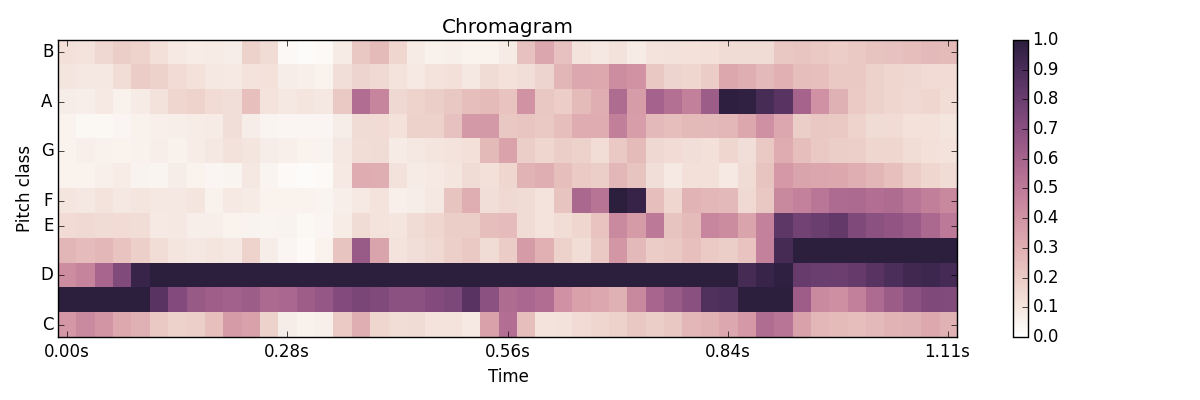
\includegraphics[width=0.7\textwidth]{../fig/chromagram1.png}
  \caption{Histogram of accuracy result from search space. Top row is baseline method 5, and the remaining rows are new feature extraction method 1, 2, and 3 respectively}
\end{figure}


\end{document}
